\documentclass{itecreport-zh}

\title{基于ONetSwitch的家庭网关设计}{A Gateway Design Basing on ONetSwitch}
\author
{贾镇远  肖法鲁  万政}
{Zhenyuan Jia,Falu Xiao,Zheng Wan}

\supervisor
{黑晓军\hspace{1em}副教授}
{Ass. Prof. Xiaojun Hei}
\date{2017}{7}{5}

\zhabstract{
	这是一个硬件课程设计实验报告。
	该硬件课程设计由 \emph{Client} 小组完成,小组成员:


	贾镇远、肖法鲁、万政


  课设中我们设计了一个家庭网关,它能通过目前高校中应用广泛的锐捷认证,支持NAT,实现多设备上网,同时还加入了适用于Linux系统的基于网络的远程监控程序,远程对该设备的状态进行监视,并进行控制。


  这样一个设备,能让我们脱离校园网单帐号,单设备的限制。
}
\zhkeywords{硬件课程设计,实验报告,网关,嵌入式Linux}

\enabstract
{
    This is a report of a hardware course design report.
    The deisgn is compeleted by the \emph{Client} group, which is made up of


    Zhenyuan Jia, Zheng Wan and Falu Xiao.


    We designed a gateway equipment, which can authenticate the Ruijie protocol. It also surport NAT, multi-device can be connect to the Internet via it. We implement a software program to get info form it and control it.


    The equipment can make multi-device conneting to the Internet, when we only have one account.
}
\enkeywords
{Hardware Course Design, Report,Gateway,Embedded Linux}

\begin{document}

\frontmatter
\maketitle
\makeabstract
\tableofcontents
% \listoffigures
% \listoftables
\mainmatter

\chapter{引言}\label{chapter:1}
\section{编写目的}\label{sec:1}
华中科技大学电信学院2014级于本学期开设硬件课程设计课程。本报告为智能路由器选题下Client小组为本次课程设计撰写的最终实验报告。
\section{背景}
华科校园网使用的是锐捷的网络认证管理方案。因此,学生使用校园网必须进行锐捷认证,而且一个校园网帐号在同一时间只允许一台设备登录校园网。这样在使用时十分不方便,而且也不能多设备同时使用上校园网。于是我们想开发一个代理设备,对校园网进行代理认证,不仅省去了每次都要登录上网的麻烦,还能多设备同时上网。
\section{课题调查}
学校的锐捷认证有两种方式:
\begin{enumerate}
    \item 802.1x认证
    \item Web认证
\end{enumerate}

如下图:

\begin{figure}[!h]
\centering
  \begin{subfigure}[b]{0.3\textwidth}
  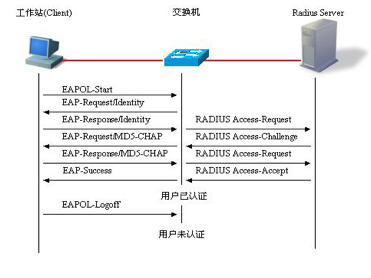
\includegraphics[width=\textwidth]{8021x.png}
  \caption{802.1x认证}
  \end{subfigure}
  ~
  \begin{subfigure}[b]{0.3\textwidth}
  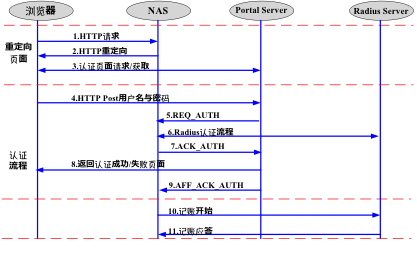
\includegraphics[width=\textwidth]{web.png}
  \caption{Web认证}
  \end{subfigure}
\end{figure}

其中802.1x集中认证是通过认证客户端向认证交换机申请认证,交换机将认证信息提交给中心认证服务器,服务器调取数据库确认认证信息的真伪,再将信息发给交换机,由交换机实际控制客户端的网络连接状态。

而Web集中认证则是增加了一个Potal服务器,提供HTTP服务,用户在WEB页面上进行认证,认证信息由Potal服务器提交给中心认证服务器,但是用户的网络连接控制还是由交换机来实现。


MentoHUST是一个支持Windows、Linux、Mac OS下的第三方锐捷认证的程序(附带支持赛尔认证)。它支持华科的锐捷认证,它是开源的项目,我们选用MentoHUST作为认证软件。


OpenWrt是适合于嵌入式设备的一个Linux发行版。相对原厂固件而言,OpenWrt不是一个单一、静态的固件,而是提供了一个可添加软件包的可写的文件系统。这使用户可以自由的选择应用程序和配置,而不必受设备提供商的限制,并且可以使用一些适合某方面应用的软件包来定制你的设备。对于开发者来说,OpenWrt是一个框架,开发者不必麻烦的构建整个固件就能得到想要的应用程序;对于用户来说,这意味着完全定制的能力,与以往不同的方式使用设备,OPKG包含超过3500个软件。

\chapter{实际开发结果}

\section{产品}
\begin{figure}[!h]
\centering
  \begin{subfigure}[b]{0.4\textwidth}
  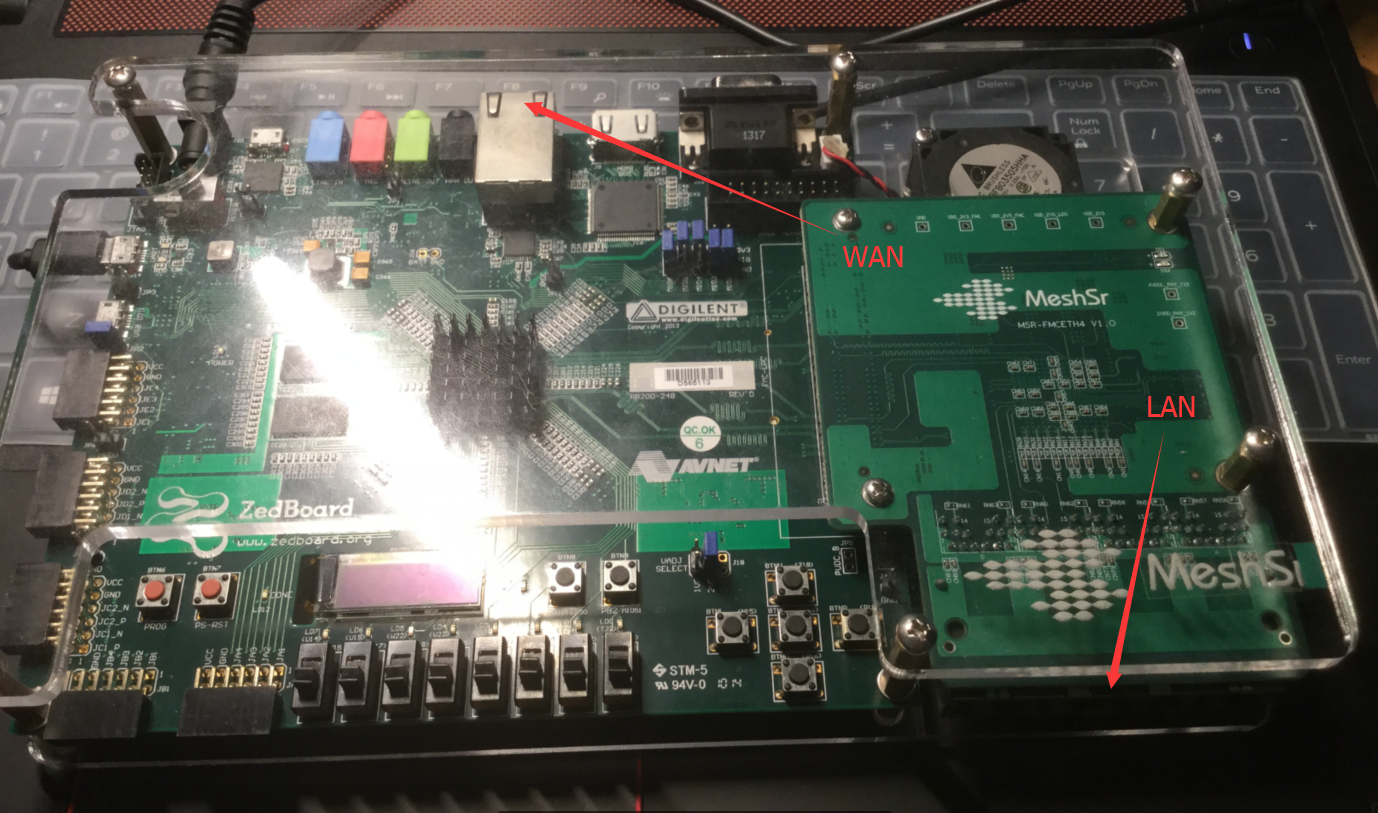
\includegraphics[width=\textwidth]{product.png}
  \caption{实物图}
  \end{subfigure}
~
  \begin{subfigure}[b]{0.4\textwidth}
  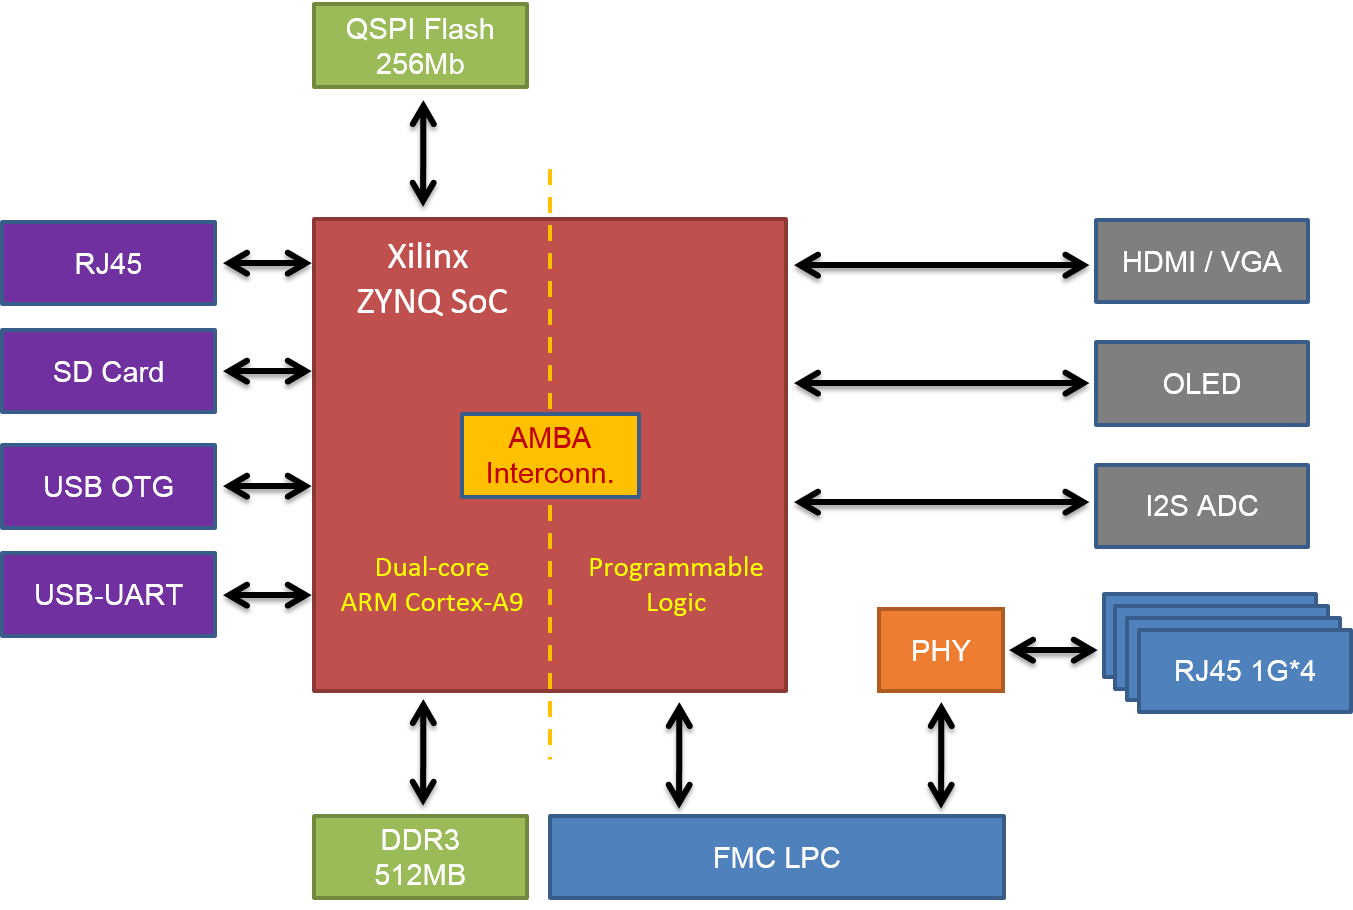
\includegraphics[width=\textwidth]{ons20-hw.png}
  \caption{结构}
  \end{subfigure}
\end{figure}
我们使用的是老师提供的ONetSwitch20开发板。该开发板母板是一块Xilinx公司的Zedboard开发板,然后通过FMC接口扩展了一块带有四个GE口的扩展板。

\begin{figure}[!h]
\centering
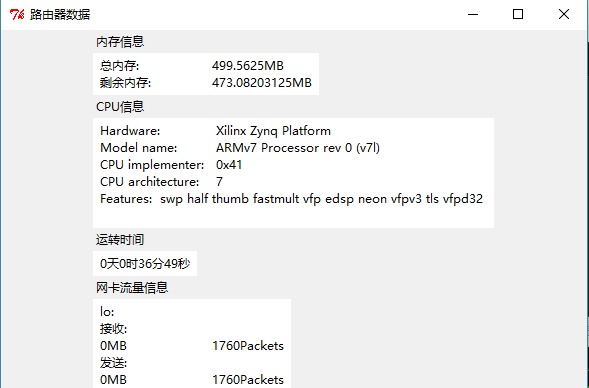
\includegraphics[width=.8\textwidth]{zynqinfo.png}
\caption{远程监视}
\end{figure}

\begin{figure}[!h]
\centering
  \begin{subfigure}[b]{0.5\textwidth}
  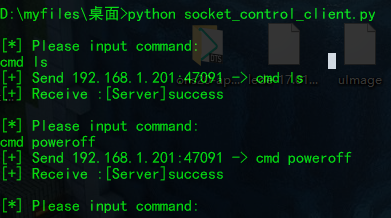
\includegraphics[width=\textwidth]{zynqctrl1.png}
  \caption{远程控制客户端}
  \end{subfigure}
  ~
  \begin{subfigure}[b]{0.4\textwidth}
  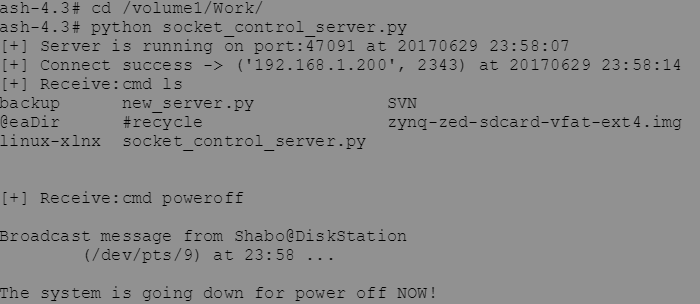
\includegraphics[width=\textwidth]{zynqctrl2.png}
  \caption{远程控制服务端}
  \end{subfigure}
\end{figure}

linux设备远程监控程序。可以根据linux设备的IP与设备通信,从而获取设备的信息或对设备进行控制。

\section{主要功能和性能}

\begin{enumerate}
    \item 校园网锐捷认证
    \item 基本的家庭网关功能
    \item 通过网络远程监控
\end{enumerate}

\begin{figure}[!h]
\centering
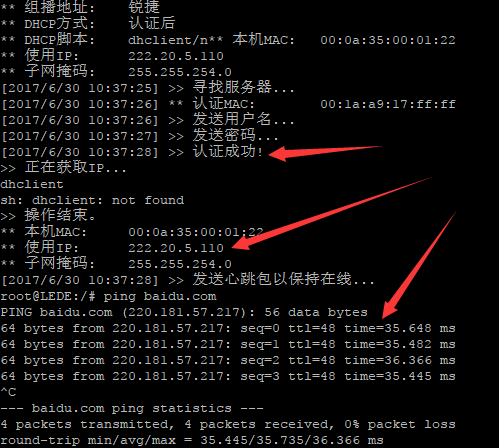
\includegraphics[width=.6\textwidth]{ruijie.png}
\caption{锐捷认证结果}
\end{figure}

开发板使用MentoHUST开源软件,能通过校园网锐捷认证,进行上网,上图认证成功并且与百度主页ping通。


母板的GE口作为wan口连上校园网,扩展版上的四个GE口作为lan口,连接内网设备。用MentoHUST锐捷认证程序在wan口进行校园网认证,电脑等终端设备接在lan口上,便可以通过开发板上网。


开发板连上网络获取IP地址之后,开启服务端程序。可以通过IP地址连接上开发板并与之通信,获取开发板的CPU负载、内存占用率、磁盘使用情况、运行时间、网络情况等数据。

\section{开发过程}
\begin{enumerate}
    \item 将OpenWRT系统刷入Zybo开发板


    我们刚开始是只有Zybo的开发板作为硬件课设的实验平台。我们发现OpenWRT项目官方对Xilinx的几块板子有支持,其中就有Zybo,于是我们将源码下载下来写入存储卡,系统成功运行。

    \item 校园网锐捷认证


    然后搭建交叉编译环境,将交叉编译出适配的MentoHUST可执行程序放入开发板,程序成功运行,并进行了锐捷认证。

    \item 将前期的工作移植到ONetSwitch20开发板上


    这里我们换了开发平台,用了叠锶公司的开源硬件平台ONetSwitch20。这个开发板母板是Xilinx的Zedborad,OpenWRT也是支持的,先将OpenWRT烧入存储卡,交叉编译,成功认证。

    \item 驱动四个扩展以太网口


    开发板扩展板有四个扩展以太网口,于是自然是要把几个以太网口驱动起来,做成多网口设备。发现官方提供了开发板的交换机例程,于是选用叠锶的BOOT.BIN、设备树文件和内核,用了LEDE的文件系统。开发板成功启动,四个以太网口也成功驱动。LEDE是成熟的特意为网络设备开发的发行版,这里可以将开发板直接配置成家庭网关。将剩下几个网口配置上IP地址,然后发现没法网络访问了,意识到是VLAN的问题————这里开发板在我的寝室内网环境下,开发板网口与内网IP段冲突了,开发板不知道包往哪个网口发送。到LEDE的网页配置,发现不支持VLAN,应该是内核没有开启802.1q支持。

    \item 重新配置编译内核,支持VLAN和NAT


    于是重新配置编译Linux内核,叠锶提供了适配的Linux源码。成功开启并配置VLAN,但是内外网是不通的。用iptables设置转发规则,发现内核不支持。再次重新编译,好在已经熟了。果然成功开启,现在基本已经是一个可用的家庭网关了。

    \item 编写远程监控程序


    我们考虑到,基础的功能虽然花费了时间精力,但是展示起来效果不太好,因为做成了基本的网关,就是连上校园网,连上设备,然后设备能通过开发板上网,没有一些amazing的效果,于是我们打算做一些应用型的功能在上面。我们想到了几套应用。
      \begin{enumerate}
        \item 一个网络摄像头的开源项目,开发板通过USB连上开发板,开发板同时通过网页将视频流送出
        \item 写一个程序,获取开发板的信息或者控制,并通过Socket通信
      \end{enumerate}
      这些想法都是很有实用价值的。但是在后面实践中,发现开发板的USB接口没法用,在固件层就没有进行连接,更改硬件工程,对USB进行驱动,剩余的时间难以完成,我们选择第二个,比较偏应用层,基本没有问题。

    \item 尝试增加wifi模块


    这里有两条路可以选择
    \begin{enumerate}
      \item 仍然尝试驱动ONetSwitch20开发板上的工作,用USBwifi模块
      \item ONetSwitch30开发板上有自带的PCIe
    \end{enumerate}

      实验室有网件的N150 USB Wi-Fi,而且OpenWRT的内核源码编译有可以加上这个模块的驱动,那么剩下的问题就是解决USB的问题。使用OpenWRT提供的固件可以驱动USB:
      \begin{figure}[!h]
      \centering
      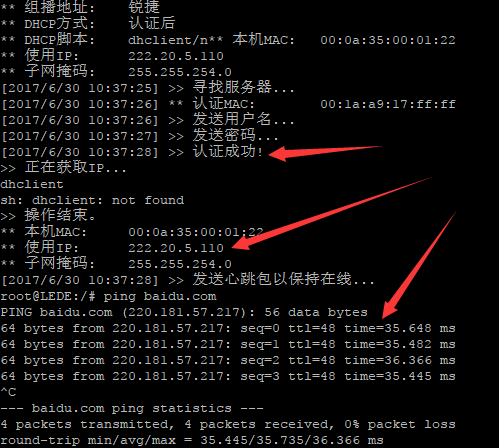
\includegraphics[width=\textwidth]{ruijie.png}
      \caption{无线网卡}
      \end{figure}
      但是还是需要解决叠锶官方固件里USB连线的问题。


      使用ONetSwitch30的PCIe-wifi模块,同样要解决固件的问题,好在官方分别提供了wifi和以太网口的tcl工程文件。相比于上一种,应该会更容易些。


      两种方案都需要从硬件工程入手,重建硬件工程,然后进行整合或者添加模块。但是官方Tcl文件运行起来还有不少BUG,折腾完了最后的时间。

\end{enumerate}
\section{部分代码}
硬件课设很多是固件层和操作系统的工作,这里展示锐捷认证和远程监控的部分主要代码。


\textbf{认证原理:}
\begin{verbatim}
================================================================
锐捷的认证过程,分为 交换机发现,用户名和密码认证,和心跳维持 三个部分。

== 交换机发现 ==

交换机发现,就是通过发送特定的数据包,找到网络上负责执行锐捷认证的那台交换机的网卡地址。

交换机发现所发送的包,是一个广播包。其广播地址在不同的版本里是不一样的。
在 v2 版本里,广播地址是标准的以太网广播包,也就是目的MAC地址 全 0 的。
在其他版本里,有需要一个特定的一个MAC地址作为广播包的目的地址。

除了地址,广播包还带有额外的数据。在 v2 版本里,这个数据由一个 “固定的数据部分”+一个随机数据 构成。 而在 v3 里,这部分数据需要从官方的客户端里进行提取。

在发送完一个广播包后,客户端等待锐捷交换机的响应,锐捷交换机会发回响应包,这样客户端就知道了锐捷交换机的 MAC 地址了 (从以太网包的发送方地址里获取)。

除了返回的响应包,一并返回的还有接下来 挑战认证协议 里需要用到的一个随机数种子。

==挑战认证协议==

锐捷使用的认证协议非常类似 HTTP 所使用的 挑战认证协议。由服务器端发回一个随机数种子,然后客户端将用户名密码和随机数种子加到一起,执行 md5 校验,并将此 md5 校验结果发给锐捷。 这么做的原因是,如果有人监听数据包截取了 md5 校验过的密码,也不能用这个 md5 的结果来替代你登录服务器。 因为每次的随机数种子是不一样的,只有真正知道密码的才能构造出合适的 md5 串来。

当然,第一部分 “服务器端发现” 的时候在广播包后面附带的数据,同样要附带在这里。这部分附加数据,是所有客户端发送的数据包都必须携带的。

锐捷检验过 md5 数值后,就会返回一个成功的数据包了,接下来就进入了心跳协议了

== 心跳协议 ==

锐捷检验过 md5 数值后,就会返回一个成功的数据包了,这个成功的数据包里,包含又一个 随机数种子。 这个随机数种子还经过了一定的混淆算法。需要首先反向解密。

解密后,每次发送心跳包钱,都将这个数字+1. 并将加1 后的数字再次加密。
解密后,再附带锐捷那一套冗长的数据,合并后的数据即可发送了。

心跳包发送频率可以控制在每分钟一个即可。
================================================================
\end{verbatim}


\textbf{MentoHUST代码:}
\begin{lstlisting}[language=C]
extern volatile int state;    //认证状态状态
extern u_char *fillBuf;     //缓冲指针

int main(int argc, char **argv)
{
#ifdef ENABLE_NLS
  textdomain(GETTEXT_PACKAGE);
  setlocale(LC_ALL, "");
#endif
  atexit(exit_handle);
  initConfig(argc, argv);/*对传入的参数进行处理*/
  /*signal函数,绑定linux信号到处理函数sig_handle,sig_handle是私有函数,对系统信号进行处理。*/
  signal(SIGALRM, sig_handle);  /* 定时器 */
  signal(SIGHUP, sig_handle);  /* 注销时 */
  signal(SIGINT, sig_handle);  /* Ctrl+C */
  signal(SIGQUIT, sig_handle);  /* Ctrl+\ */
  signal(SIGTSTP, sig_handle);  /* Ctrl+Z */
  signal(SIGTERM, sig_handle);  /* 被结束时 */
  if (dhcpMode == 3)    /* 认证前DHCP */
    switchState(ID_DHCP);
  else
    switchState(ID_START);  /* 开始认证 */

/*主函数调用pcap_loop函数,进入循环,不断抓包进行判断。*/
  if (-1 == pcap_loop(hPcap, -1, pcap_handle, NULL)) { /* 开始捕获数据包 */
    printf(_("!! 捕获数据包失败,请检查网络连接!\n"));
#ifndef NO_NOTIFY /*消息显示功能,需呀libnotify库*/
    if (showNotify && show_notify(_("MentoHUST - 错误提示"),
      _("捕获数据包失败,请检查网络连接!"), 1000*showNotify) < 0)
      showNotify = 0;
#endif
  }
  exit(EXIT_FAILURE);
}

\*MentoHUST使用的libpcap库,下面是libpcap处理函数,抓到包之后根据包内信息判断认证状态。
再将得到的状态传给switchState()函数*\
static void pcap_handle(u_char *user, const struct pcap_pkthdr *h, const u_char *buf)
{
  static unsigned failCount = 0;
#ifndef NO_ARP
  if (buf[0x0c]==0x88 && buf[0x0d]==0x8e) {
#endif
    if (memcmp(destMAC, buf+6, 6)!=0 && startMode>2)  /* 服务器MAC地址不符 */
      return;
    capBuf = buf;
    if (buf[0x0F]==0x00 && buf[0x12]==0x01 && buf[0x16]==0x01) {  /* 验证用户名 */
      if (startMode < 3) {
        memcpy(destMAC, buf+6, 6);
        printf(_("** 认证MAC:\t%s\n"), formatHex(destMAC, 6));
        startMode += 3; /* 标记为已获取 */
      }
      if (startMode==3 && memcmp(buf+0x17, "User name", 9)==0)  /* 塞尔 */
        startMode = 5;
      switchState(ID_IDENTITY);
    }
    else if (buf[0x0F]==0x00 && buf[0x12]==0x01 && buf[0x16]==0x04) /* 验证密码 */
      switchState(ID_CHALLENGE);
    else if (buf[0x0F]==0x00 && buf[0x12]==0x03) {  /* 认证成功 */
      printf(_(">> 认证成功!\n"));
      failCount = 0;
      if (!(startMode%3 == 2)) {
        getEchoKey(buf);
        showRuijieMsg(buf, h->caplen);
      }
      if (dhcpMode==1 || dhcpMode==2) /* 二次认证第一次或者认证后 */
        switchState(ID_DHCP);
      else if (startMode%3 == 2)
        switchState(ID_WAITECHO);
      else
        switchState(ID_ECHO);
    }
    else if (buf[0x0F]==0x00 && buf[0x12]==0x01 && buf[0x16]==0x02) /* 显示赛尔提示信息 */
      showCernetMsg(buf);
    else if (buf[0x0F] == 0x05) /* (赛尔)响应在线 */
      switchState(ID_ECHO);
    else if (buf[0x0F]==0x00 && buf[0x12]==0x04) {  /* 认证失败或被踢下线 */
      if (state==ID_WAITECHO || state==ID_ECHO) {
        printf(_(">> 认证掉线,开始重连!\n"));
        switchState(ID_START);
      }
      else if (buf[0x1b]!=0 || startMode%3==2) {
        printf(_(">> 认证失败!\n"));
        if (startMode%3 != 2)
          showRuijieMsg(buf, h->caplen);
        if (maxFail && ++failCount>=maxFail) {
          printf(_(">> 连续认证失败%u次,退出认证。\n"), maxFail);
          exit(EXIT_SUCCESS);
        }
        restart();
      }
      else
        switchState(ID_START);
    }
#ifndef NO_ARP
  } else if (gateMAC[0]!=0xFE && buf[0x0c]==0x08 && buf[0x0d]==0x06) {
    if (*(u_int32_t *)(buf+0x1c) == gateway) {
      char str[50];
      if (gateMAC[0] == 0xFF) {
        memcpy(gateMAC, buf+0x16, 6);
        printf(_("** 网关MAC:\t%s\n"), formatHex(gateMAC, 6));
        sprintf(str, "arp -s %s %s", formatIP(gateway), formatHex(gateMAC, 6));
        system(str);
      } else if (buf[0x15]==0x02 && memcmp(&rip, buf+0x26, 4)==0
        && memcmp(gateMAC, buf+0x16, 6)!=0) {
        printf(_("** ARP欺骗:\t%s\n"), formatHex(buf+0x16, 6));
#ifndef NO_NOTIFY
        if (showNotify) {
          sprintf(str, _("欺骗源: %s"), formatHex(buf+0x16, 6));
          if (show_notify(_("MentoHUST - ARP提示"), str, 1000*showNotify) < 0)
            showNotify = 0;
        }
#endif
      }
    }
  }
#endif
}

\*若状态不变,计数器加一,判断是否超时,根据状态判断超时原因。
若状态改变,返回下一状态处理函数*\
int switchState(int type)
{
  if (state == type) /* 跟上次是同一状态? */
    sendCount++;
  else
  {
    state = type;
    sendCount = 0;
  }
  if (sendCount>=MAX_SEND_COUNT && type!=ID_ECHO)  /* 超时太多次? */
  {
    switch (type)
    {
    case ID_START:
      printf(_(">> 找不到服务器,重启认证!\n"));
      break;
    case ID_IDENTITY:
      printf(_(">> 发送用户名超时,重启认证!\n"));
      break;
    case ID_CHALLENGE:
      printf(_(">> 发送密码超时,重启认证!\n"));
      break;
    case ID_WAITECHO:
      printf(_(">> 等候响应包超时,自行响应!\n"));
      return switchState(ID_ECHO);
    }
    return restart();
  }
  switch (type)
  {
  case ID_DHCP:
    return renewIP();
  case ID_START:
    return sendStartPacket();
  case ID_IDENTITY:
    return sendIdentityPacket();
  case ID_CHALLENGE:
    return sendChallengePacket();
  case ID_WAITECHO: /* 塞尔的就不ping了,不好计时 */
    return waitEchoPacket();
  case ID_ECHO:
    if (pingHost && sendCount*echoInterval > 60) {  /* 1分钟左右 */
      if (isOnline() == -1) {
        printf(_(">> 认证掉线,开始重连!\n"));
        return switchState(ID_START);
      }
      sendCount = 1;
    }
#ifndef NO_ARP
    if (gateMAC[0] != 0xFE)
      sendArpPacket();
#endif
    return sendEchoPacket();
  case ID_DISCONNECT:
    return sendLogoffPacket();
  }
  return 0;
}
\end{lstlisting}





\textbf{Linux信息获取代码:}
\begin{lstlisting}[language=Python]
#getinfo-srv.py
def tcplink(sock, addr):
#Linux状态获取函数直接读取/proc目录下文件获取数据,或者调用Python相关库
    def memory_stat(): #获取磁盘数据

    def cpu_stat(): #获取CPU状态

    def net_stat(): #获取网络状态

    def uptime_stat(): #获取运行时间

    def disk_stat():  #磁盘使用空间,单位Byte
    #将数据组织成dict结构
    sendpacket = {'cpu_stat':cpu_stat(), 'mem_stat':memory_stat(), 'net_stat':net_stat(), 'runtime_stat':uptime_stat(), 'disk_stat':disk_stat()}
    #将dict转换成str发送
    sock.send(str(sendpacket))
    time.sleep(1)

#socket
s = socket.socket(socket.AF_INET, socket.SOCK_STREAM)
s.bind(('0.0.0.0', 9999))
s.listen(5)
print('Waiting for connection...')

while True:
    sock, addr = s.accept()
    
    while True:
        tcplink(sock, addr)

#-----------------------------------------------------------------#
#getinfo-clt.py
def get_info():
    # global server_list
    server = '192.168.1.1'
    connPort = 9999
    # readtarget()
    connserver(server, connPort)

def connserver(host, port):
    s = socket.socket(socket.AF_INET, socket.SOCK_STREAM)
    s.connect((host, port))
    while True:
        buf = s.recv(4096)
        if not len(buf):
            break

        def netstat_proc(info):
            resu = ''
            for di in info:
                resu = resu+str(di['interface'])+':\n接收:\n'+str(di['ReceiveBytes']/1048576)+'MB\t\t'+str(di['ReceivePackets'])+'Packets\n发送:\n'+str(di['TransmitBytes']/1048576)+'MB\t\t'+str(di['TransmitPackets'])+'Packets\n\n'
            return resu
        info = eval(str(buf).strip('\n'))#将str再转换回dict结构
        #分别存储CPU、磁盘等的输出信息
        global buf1
        global buf2
        global buf3
        global buf4
        global buf5
        buf1 = '总内存:\t\t'+str(info['mem_stat']['MemTotal']/1048576)+'MB\n剩余内存:\t\t'+str(info['mem_stat']['MemFree']/1048576)+'MB'
        buf2 = 'Hardware:\t'+cst['Hardware']+'Model name:\t'+cst['model name']+'CPU implementer:\t'+cst['CPU implementer']+'CPU architecture:\t'+cst['CPU architecture']+'Features:\t'+cst['Features']
        buf3 = str(info['runtime_stat']['day'])+'天'+str(info['runtime_stat']['hour'])+'时'+str(info['runtime_stat']['minute'])+'分'+str(info['runtime_stat']['second'])+'秒'#).strip('\n')
        buf4 = netstat_proc(info['net_stat'])
        buf5 = 'Available:\t\t'+str(info['disk_stat']['available']/1048576)+'GB\nUsed:\t\t'+str(info['disk_stat']['used']/1048576)+'GB\nCapacity:\t\t'+str(info['disk_stat']['capacity']/1048576)+'GB'
#info['cpu_stat']['vendor_id'] + 

if __name__ == "__main__":
    # server_list = []
    buf1 = ""
    buf2 = ""
    buf3 = ""
    buf4 = ""
    buf5 = ""
    t1 = threading.Thread(target = main_window, args = ())#图形界面的线程
    t2 = threading.Thread(target = get_info, args = ())#数据获取线程
    t1.start()
    t2.start()
    t1.join()
    t2.join()
\end{lstlisting}





\textbf{Linux控制代码:}
\begin{lstlisting}[language=Python]
#ctrl-srv.py
def parsecmd(strings):
    midsplit = str(strings).split(" ")
    if len(midsplit) >= 2 and midsplit[0] == "cmd":#检测命令头是否有cmd防止出错
        try:
            command = subprocess.Popen(strings[4:], shell=True)
            command.communicate()
            print "\n"
        except Exception, e:
            print e.message
            traceback.print_exc()

def recvdata(port):
    s = socket.socket(socket.AF_INET, socket.SOCK_STREAM)#创建套接字
    s.setsockopt(socket.SOL_SOCKET, socket.SO_REUSEADDR, 1)
    s.bind(('', port))#绑定
    s.listen(1)#监听端口
    print "[+] Server is running on port:%s at %s" % (str(port), time.strftime("%Y%m%d %H:%M:%S", time.localtime()))
    while True:
        mainsocket, mainhost = s.accept()
        print "[+] Connect success -> %s at %s" % (str(mainhost), time.strftime("%Y%m%d %H:%M:%S", time.localtime()))
        if mainhost:
            while True:
                data = mainsocket.recv(1024)
                if data:
                    print "[+] Receive:%s" % data
                    mainsocket.sendall("[Server]success")
                    parsecmd(data)
                if data == "close session":
                    mainsocket.close()
                    print "[+] Quit success"
                    break
            break


if __name__ == "__main__":
    # some public variable
    connPort = 47091
    onethreads = threading.Thread(target=recvdata, args=(connPort,))
    onethreads.start()

#-----------------------------------------------------------------#
#ctrl-client.py
def connserver(host, port):
    s = socket.socket(socket.AF_INET, socket.SOCK_STREAM)
    s.connect((host, port))
    while True:
        print "\n[*] Please input command:"
        data = raw_input()#获取输入指令
        if not data:
            break
        s.sendall(data)#发送
        recvdata = s.recv(1024)
        print "[+] Send %s:%s -> %s" % (host, str(connPort), data)
        time.sleep(0)
        if recvdata:
            print "[+] Receive :%s" % recvdata
        if data == "close session":
            s.close()
            break

if __name__ == "__main__":
    host = '192.168.1.201'
    connPort = 47091

    connserver(host, connPort)#连接对应服务端
\end{lstlisting}
\chapter{开发工作评价}
\section{对产品质量的评价}
总的来说,最终的成品大体上是达到了可用的程度,如果直接拿到宿舍,能够日常使用,但是欠缺的地方还很多。有以下一些点:
\begin{enumerate}
  \item 没有wifi模块。相比于我自己用的路由器,这个东西最大的缺点就是没有wifi模块。这方面确实工作量比较大,最后的时间不太够,但是思路应该是对的,只是在碰到的问题上需要慢慢打磨。
  \item 远程监控程序过于简陋。信息获取和控制两个程序,没有整合到一起,这对使用十分不方便。界面和功能上都十分简陋,如果日常使用,这个肯定是不够的。
\end{enumerate}
\section{组内成员评价}
组内打分:
\begin{enumerate}
  \item 贾镇远:90分
  \item 万政:85分
  \item 肖法鲁:85分
\end{enumerate}
\chapter{经验与教训}
本次课程设计,学到了很多东西。以前虽然也学了嵌入式的课程,也知道Bootloader,知道它的作用,但这些理解很抽象。在这次硬件课设中,我们对固件层、操作系统层和应用层都有接触,亲自编译内核,亲自制作嵌入式系统的启动分区。然后我们对嵌入式系统的启动流程和需要的文件,各文件的作用有了比以前更深、更具体的理解。


以前我们使用Linux系统,只是使用,对整个系统的组成、Linux Kernel和文件系统之间是怎样的一个关系,都只有一个模糊的概念,知道些东西,但无法表达,不能算真正的理解。这些概念,现在,不再模糊。


另一方面,在整个过程中,碰到的问题其实是比较多的,在这样一个不断找到问题根源,然后解决问题的过程中,我想我们更是得到了解决问题的通用方法,那就是查资料、找懂的人同时还必须具有耐心。也许这些还不完全,但确实能在碰到问题时给我们许多帮助。


此次硬件课设让我感到遗憾的地方也有很多。我自己感觉这次硬件课设好像不同于上学期的软件课设。这次课设,很多时候我们都使用了别人给出的东西,开源的代码、官方给好的固件,最后拼凑成一个产品,只有最后的Python程序,是自己创造的东西。这让我心里有一种空落落的感觉,不同于上学期,从零构建一个软件工程的那种满足感。但实际上,我们所使用的那些东西,如果完全由我们自己来完成,可能吗?不可能。只说OpenWRT,就完全不可能由我们重写一个。


但是仔细想想,或许,我需要的是一个思维的转变。


到了路由器这个量级的产品,涉及的东西太多了,从硬件到操作系统,到软件,已经没办法自己独立完成了,该用的东西还得用,将别人的工作整合到一起也是一种创新,也有自己的工作量。
况且,上学期写邮件客户端,也是调用了Python的各种库,底层的网络通信过程也是别人做好的封装,同样是用了别人的东西。


现在的开发过程已经不同于我初学的时候,写的都是简单的程序,老师布置的作业,都是独自完成。如果自己要做一个完整的复杂一点的东西,已经不可能自己从零开始了,不实际,也没必要。“不要重复造轮子”,就是这样一个道理。就是要学会使用工具。


这次硬件课设,给我们的这些感悟,以后,将成为我们的助力。
\end{document}


